% ----- APPENDIX B ------------------%
%
% Definition of labels and variables %
% ---------------------------------- %
\chapter{Definitions and Conventions}
\label{app:variables}

\begin{figure}[!h]
\centerline{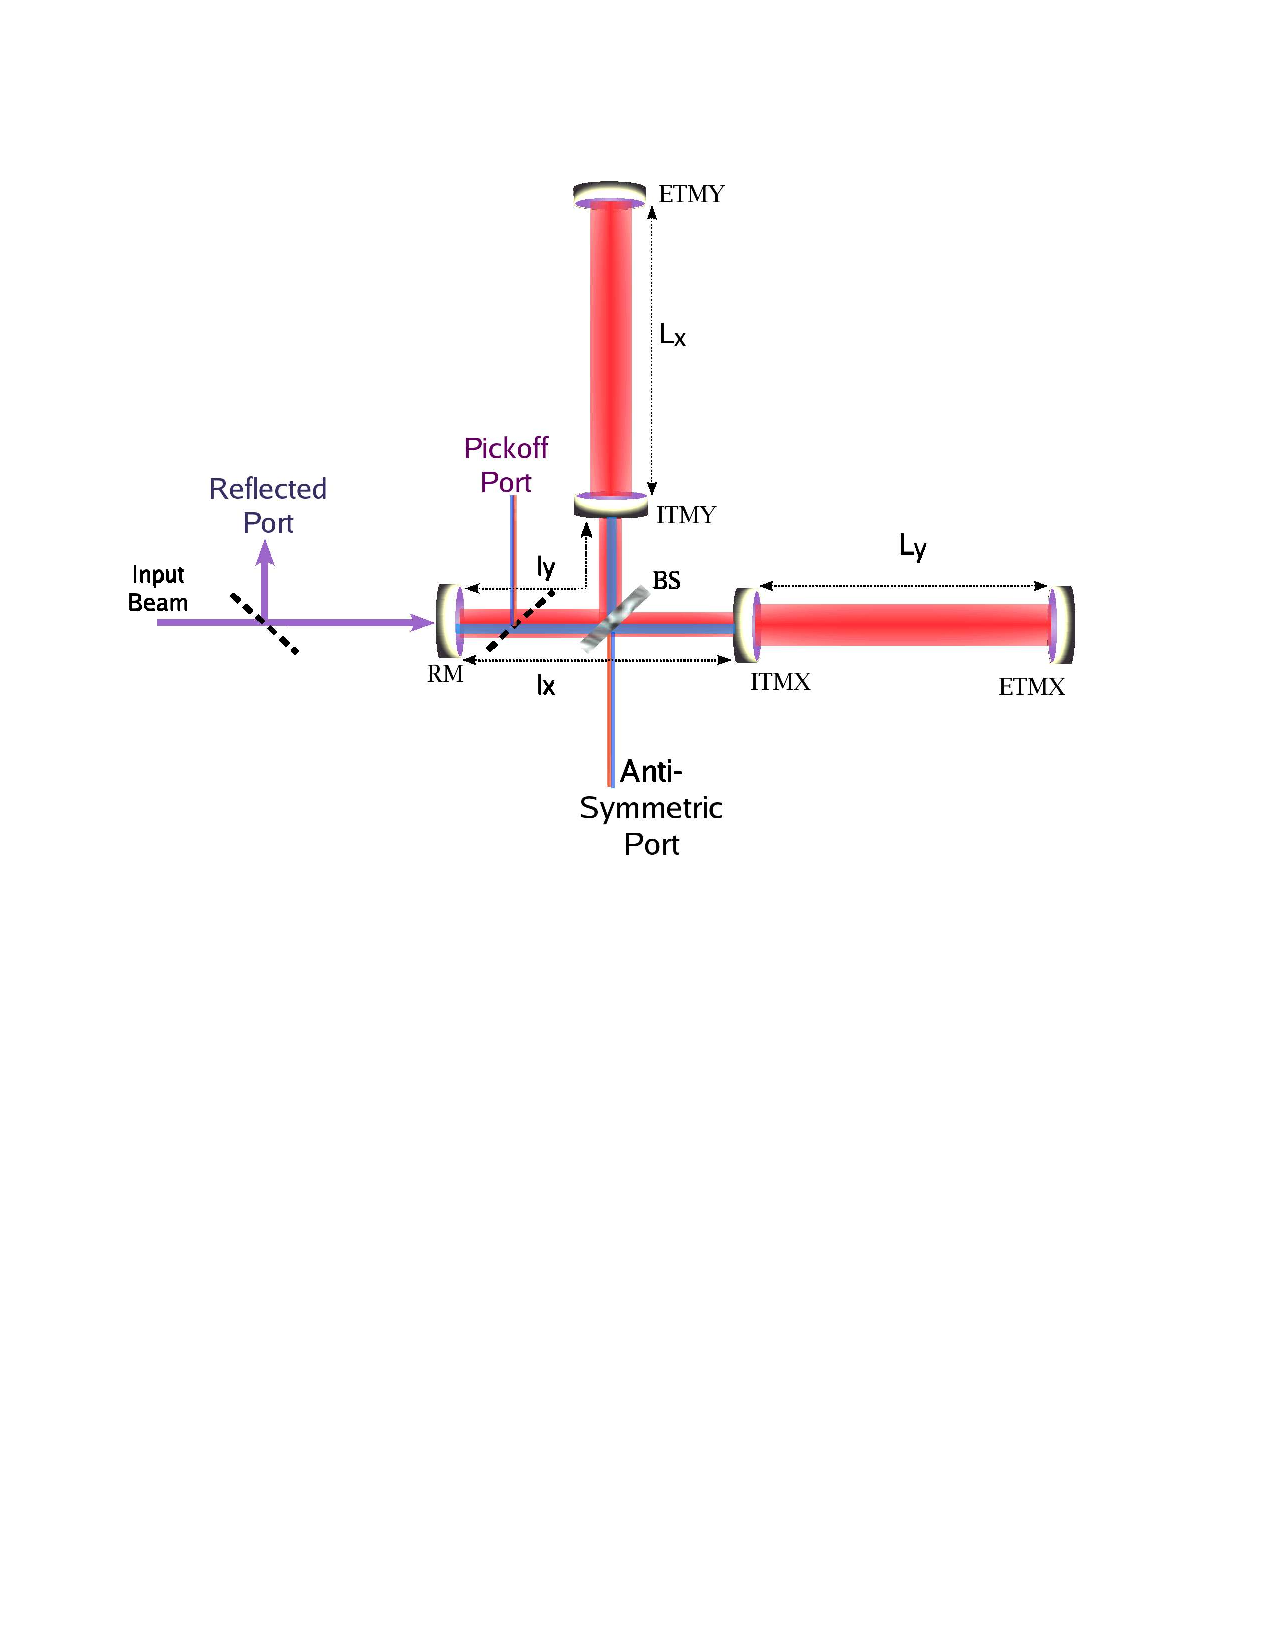
\includegraphics[angle=0,width=6.5in]{Figures/Chap3/IFO2.pdf}}
\end{figure}

The interferometer output signals are naturally represented in basis which
separates common and differential lengths:

\begin{alignat}{2} \label{eq:LengthDefinitions}
    L_{+} &= \frac{L_y + L_x}{2}      & \qquad     L_{-} &= L_y - L_x \\
    l_{+} &= \frac{l_y + l_x}{2}      & \qquad     l_{-} &= l_y - l_x
 \notag
\end{alignat}
It is a little awkward that there's a factor of 2 difference between how common
and differential lengths are defined. It is this way because we generally are
interested in the \emph{average} of the two arms. On the other hand, in the
literature, strain is usually defined as 

\begin{equation}
h \equiv \frac{L_y-L_x}{L_{+}}
\end{equation}
Most of the conventions in this thesis for defining reflectivities, lengths,
etc. follow \cite{Sigg:FreqResp}. They are restated here for convenience.

There is a convention followed for macroscopic lengths and microscopic lengths.
The use of $\Delta$ or $\delta$ implies a microscopic deviation from resonance,
whereas the lack of either implies a macroscopic length. The upper case, $\Delta$,
is used to imply a static or quasi-static shift from resonance. The lower case,
$\delta$, is used to denote a quantity fluctuating at AC, in the GW band.

The variable naming convention for reflection and transmission coefficients and
cavity gain coefficients is that the lower case variables ($r$, $t$, and $g$) 
refer to amplitude coefficients and the upper case ($R$, $T$, and $G$) is for
power. So, e.g. $R = r^2$.

On resonance, the amplitude reflectivity of an arm for the carrier is

\begin{equation}
r_c = \frac{r_{\mbox{\tiny ITM}} - r_{\mbox{\tiny ETM}}}
           {1 - r_{\mbox{\tiny ITM}} r_{\mbox{\tiny ETM}}}
\label{eq:arm_reflectivity}
\end{equation}
where $r_{\mbox{\tiny ITM}}$ and $r_{\mbox{\tiny ETM}}$ are the amplitude 
reflectivity of the Input Test Mass and the End Test Mass, respectively. 
For the LIGO interferometers, $r_{\mbox{\tiny ETM}} > r_{\mbox{\tiny ITM}}$, 
and so $r_c$ is negative. So as the cavity shifts from
off resonance to on resonance the reflected field gets a sign flip, but has
nearly the same amplitude. This is because the leakage field from the
cavity has $\sim$twice the amplitude but the opposite sign as the field
promptly reflected from the input mirror.

The RF sidebands are almost exactly anti-resonant in the arm cavities, so the
reflectivity of the combined Fabry-Perot Michelson for the sidebands is 
determined entirely by the Schnuup asymmetry:

\begin{equation}
r_M = cos \frac{2 \, \omega_m \, l_{-}}{c}
\end{equation}
Also frequently used is, $r_c'$, the derivative of the arm cavity reflectivity
with respect to the round trip phase,$\phi$, evaluated at $2 \pi$:

\begin{equation}
r_c' = \frac{(1-r_{\mbox{\tiny ITM}}^2)r_{\mbox{\tiny ETM}}}
            {(1-r_{\mbox{\tiny ITM}}r_{\mbox{\tiny ETM}})^2}
\end{equation}
In Equations~\ref{eq:recyclinggains}, the amplitude transmission to the
anti-symmetric port, the reflectivities for the entire interferometer, and the
recycling cavity's recycling gains for the carrier and the sideband are defined.

\begin{alignat}{2}\label{eq:recyclinggains}
t_{cr} &= 0                  & \qquad     
t_{sb} &= \frac{t_{\mbox{\tiny RM}}t_{\mbox{\tiny M}}}{1-r_{\mbox{\tiny RM}}r_{\mbox{\tiny M}}} \\
r_{cr} &= \frac{r_{\mbox{\tiny RM}}+r_c}{1+r_{\mbox{\tiny RM}}r_c} & \qquad 
r_{sb} &= \frac{r_{\mbox{\tiny RM}}-r_{\mbox{\tiny M}}}{1-r_{\mbox{\tiny RM}}r_{\mbox{\tiny M}}} \notag \\
g_{cr} &= \frac{t_{\mbox{\tiny RM}}}{1+r_{\mbox{\tiny RM}}r_c}   & \qquad  
g_{sb} &= \frac{t_{\mbox{\tiny RM}}}{1-r_{\mbox{\tiny RM}}r_{\mbox{\tiny M}}} \notag
\end{alignat}
Also, since most of the measured signals are proportional to the product of the carrier
and sideband field, a standard pre-factor is defined which is included in almost all
of the sensing matrix elements:

\begin{equation}
  \aleph = 4 J_0(\Gamma) J_1(\Gamma) P_{in}
\end{equation}












